% 8 variables in here:
% u_1 = -2.9, h_1 = 8.8, U_1 = -1.7, H_1 = 10.6, u_2 = -1.4, h_2 = 9.1, U_2 = 3.8, H_2 = 11.6
\begin{figure}[ht]
\centering
  \subfloat[Momentum of point $p_1^L$] {
    %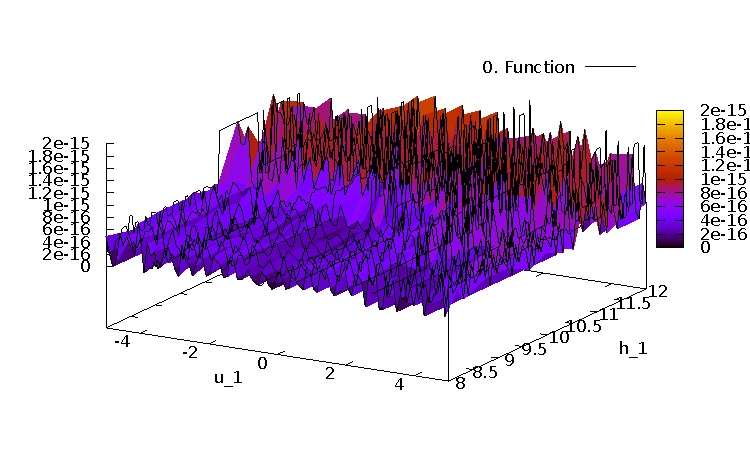
\includegraphics[scale=\zoomfactor]{{{2_random_new/x_y_-1.7_10.6_-1.4_9.1_3.8_11.6f0}}}  
    \begin{tikzpicture}
      \node at (0,0) {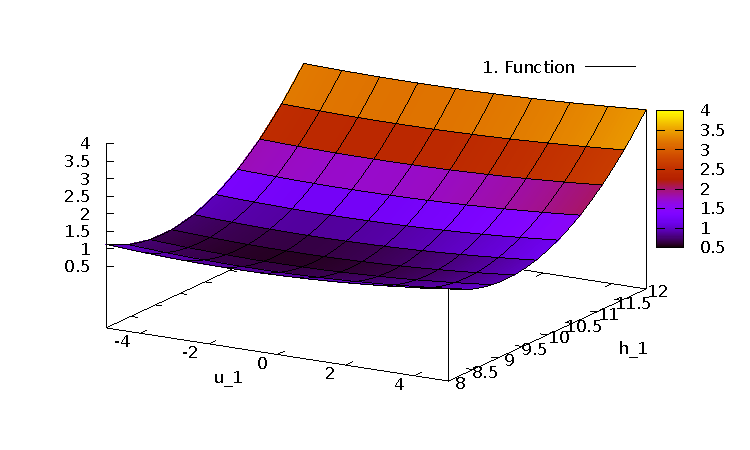
\includegraphics[scale=\zoomfactor]{{{2_random_new/x_y_-1.7_10.6_-1.4_9.1_3.8_11.6f1}}}  };
      \fill[white] (.8,1.2) rectangle (1.75,1.5);
      \node[align=right, text width=3cm] at (.2,1.33) {\textsf{\tiny{Momentum error}}};
    \end{tikzpicture}
  }
  \subfloat[Momentum of point $p_2^L$] {
    %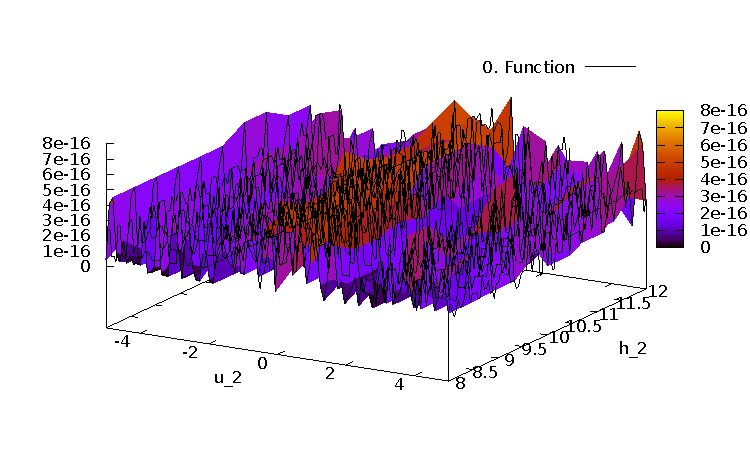
\includegraphics[scale=\zoomfactor]{{{2_random_new/-2.9_8.8_-1.7_10.6_x_y_3.8_11.6f0}}}  
    \begin{tikzpicture}
      \node at (0,0) {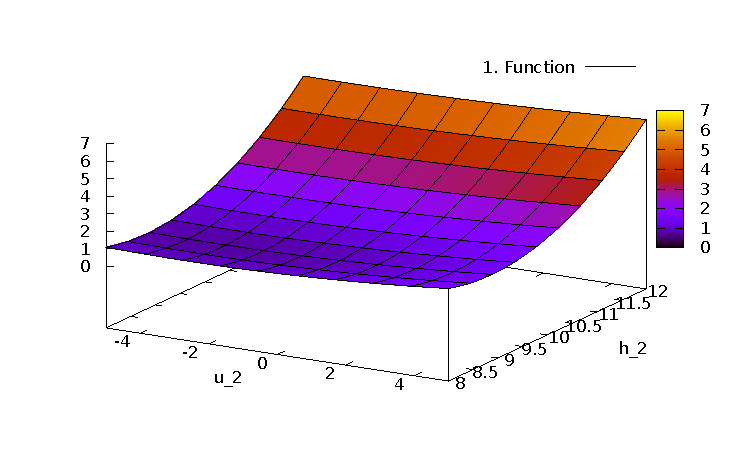
\includegraphics[scale=\zoomfactor]{{{2_random_new/-2.9_8.8_-1.7_10.6_x_y_3.8_11.6f1}}}  };
      \fill[white] (.8,1.2) rectangle (1.75,1.5);
      \node[align=right, text width=3cm] at (.2,1.33) {\textsf{\tiny{Momentum error}}};
    \end{tikzpicture}
  }

  \subfloat[Momentum of point $p_1^R$] {
    %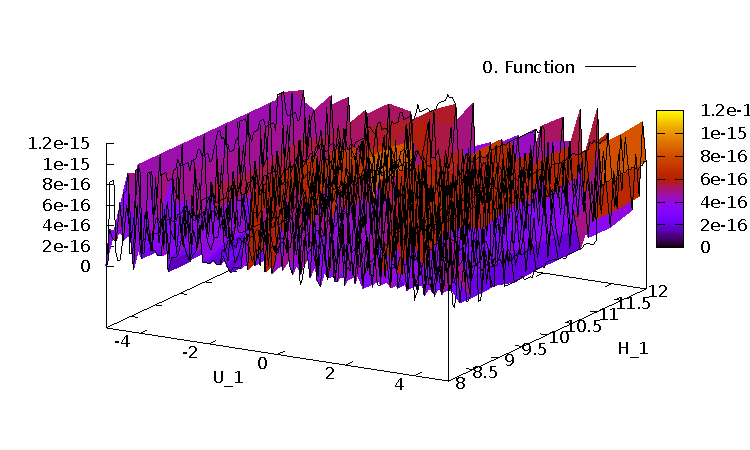
\includegraphics[scale=\zoomfactor]{{{2_random_new/-2.9_8.8_x_y_-1.4_9.1_3.8_11.6f0}}}  
    \begin{tikzpicture}
      \node at (0,0) {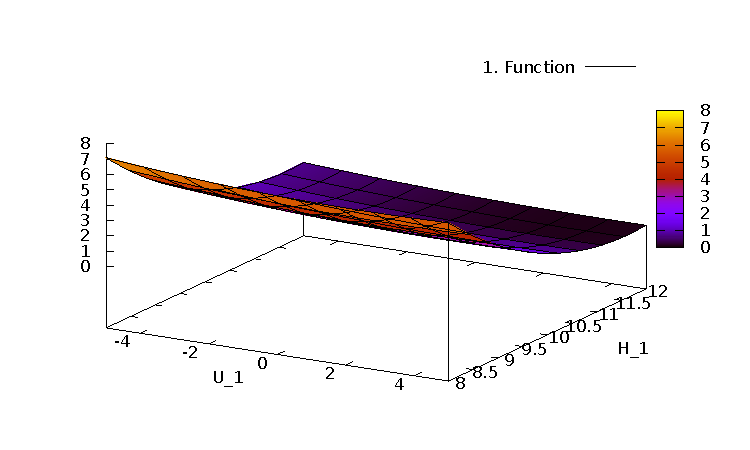
\includegraphics[scale=\zoomfactor]{{{2_random_new/-2.9_8.8_x_y_-1.4_9.1_3.8_11.6f1}}}  };
      \fill[white] (.8,1.2) rectangle (1.75,1.5);
      \node[align=right, text width=3cm] at (.2,1.33) {\textsf{\tiny{Momentum error}}};
    \end{tikzpicture}
  }
  \subfloat[Momentum of point $p_2^R$] {
    %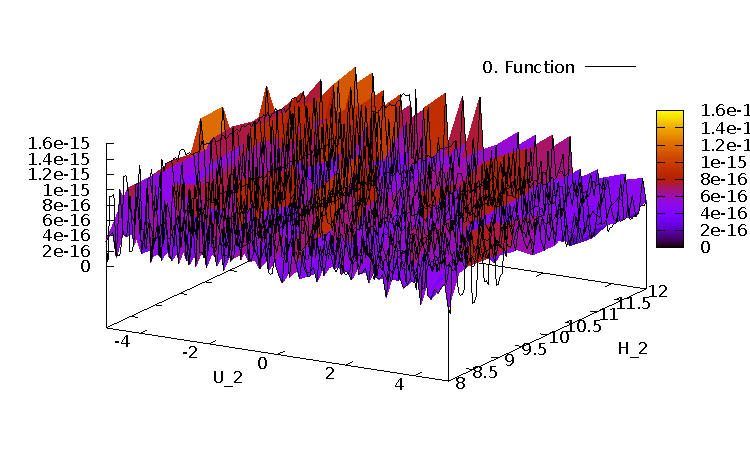
\includegraphics[scale=\zoomfactor]{{{2_random_new/-2.9_8.8_-1.7_10.6_-1.4_9.1_x_yf0}}}  
    \begin{tikzpicture}
      \node at (0,0) {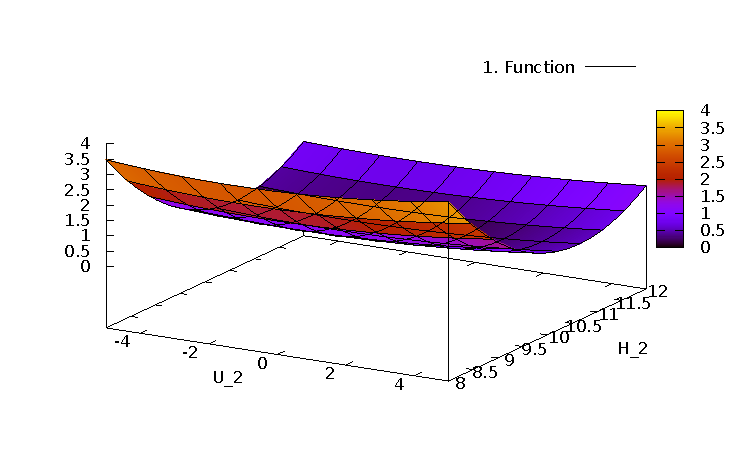
\includegraphics[scale=\zoomfactor]{{{2_random_new/-2.9_8.8_-1.7_10.6_-1.4_9.1_x_yf1}}}  };
      \fill[white] (.8,1.2) rectangle (1.75,1.5);
      \node[align=right, text width=3cm] at (.2,1.33) {\textsf{\tiny{Momentum error}}};
    \end{tikzpicture}
  }
  \caption{Two points for each triangle. Values for the points are: $u_1^L = -2.9, h_1^L = 8.8, u_1^R = -1.7, h_1^R = 10.6, u_2^L = -1.4, h_2^L = 9.1, u_2^R = 3.8, h_2^r = 11.6$.}
  \label{fig:two-points-random}
\end{figure}

%%% Local Variables:
%%% TeX-master: "../results.tex"
%%% End:

%%% Local Variables:
%%% TeX-master: "../results.tex"
%%% End:
